\subsection{Results on the DECam survey}
\label{sec:results_on_decam}

We next demostrate StarNet on a larger region of the sky.
The DECAPS survey imaged stars in our own Milky Way, and we chose
a $4000 \times 2000$ frame centered at coordinates $\text{RA} = 266.044^\circ$ and
$\text{DEC} = -28.88111^\circ$. See Figure~\ref{fig:decaps} for an example image.

The DECAPS image is somewhat sparser than M2.
Thus, we set the Poisson mean parameter of the star density lower smaller than on M2 to fifty stars per 100 x 100 pixel image.
We used a tile size of $10\times 10$ pixels with $20\times20$-pixel
padded tiles. 
We produced
a catalog for the full $4000 \times 1000$ frame, consisting of $9,000$ stars. 
The color-magnitude diagram clearly shows a sequence of blue
stars that are reddened at fainter magnitudes. 

With the smaller density of stars, 
the SGD algorithm converged after only 100 epochs; 
the fit took ten minutes. After the fit, producing the catalog 
took only two seconds. 
On the other hand, extrapolating the runtime of PCAT, running MCMC on the same frame
would take on the order of day.


\begin{figure}[!htb]
    \centering
    \begin{subfigure}[T]{0.45\textwidth}
    \centering
    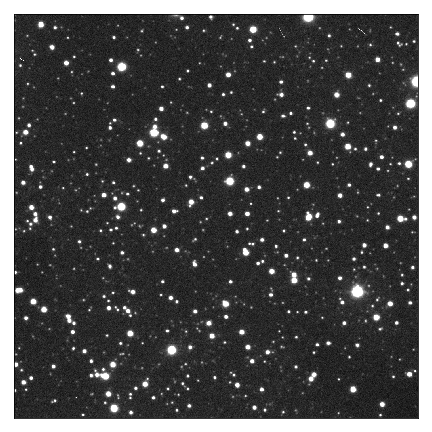
\includegraphics[width=\textwidth]{./figures/decaps/example_subimage1000_decaps.png}
    \end{subfigure}
    \hfill
    \begin{subfigure}[T]{0.5\textwidth}
    \centering
    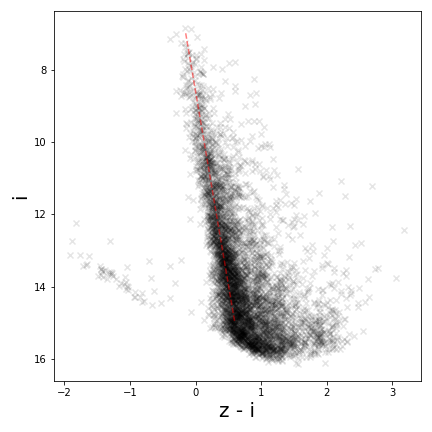
\includegraphics[width=\textwidth]{./figures/decaps/decaps_cmd.png}
    \end{subfigure}
    \caption{(Left) A 1000 x 1000 pixel subregion of the DECAM survey. 
    (Right) Color magnitude diagram for the Decaps image. Red dashed line highlights
    the inferred blue main-sequence stars}
    \label{fig:decaps}
\end{figure}

% \begin{figure}[tb]
%     \centering
%     \includegraphics[width=0.8\textwidth]
%     \vspace{-0.4cm}
%     \caption{A 1000 x 1000 pixel subregion of the DECAM survey. }
%     \label{fig:decaps_ex}
% \end{figure}

% \begin{figure}[tb]
%     \centering
%     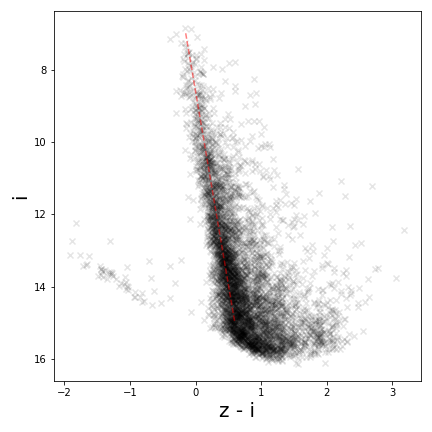
\includegraphics[width=0.4\textwidth]{./figures/decaps/decaps_cmd.png}
%     \vspace{-0.4cm}
%     \caption{Color magnitude diagram for the Decaps image. Red dashed line highlights
%     the inferred blue main-sequence stars.
%     }
%     \label{fig:decaps_cmd}
% \end{figure}
